\section{Spline Class Reference}
\label{classSpline}\index{Spline@{Spline}}
{\tt \#include $<$spline.h$>$}

Inheritance diagram for Spline::\begin{figure}[H]
\begin{center}
\leavevmode
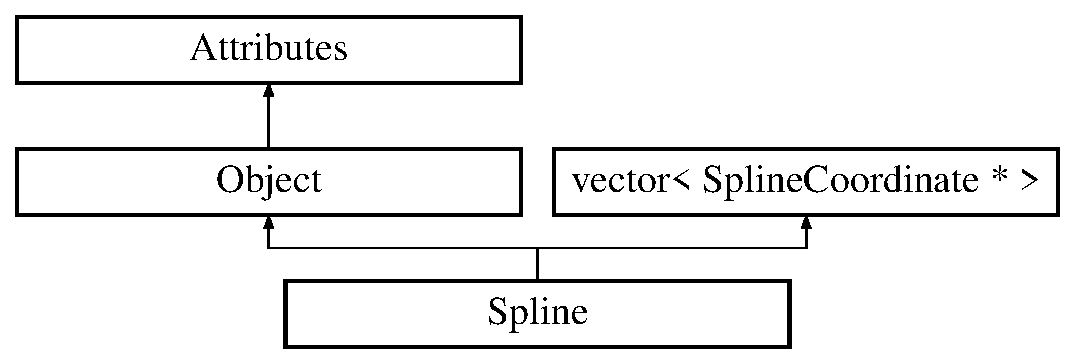
\includegraphics[height=3cm]{classSpline}
\end{center}
\end{figure}
\subsection*{Public Types}
\begin{CompactItemize}
\item 
enum {\bf Sub\-Types} \{ {\bf Opened}, 
{\bf Closed}
 \}
\end{CompactItemize}
\subsection*{Public Methods}
\begin{CompactItemize}
\item 
{\bf Spline} ()
\item 
{\bf Spline} ({\bf Spline\-Coordinate} $\ast$, {\bf Spline\-Coordinate} $\ast$)
\item 
{\bf $\sim$Spline} ()
\item 
void {\bf set\-Sub\-Type} ({\bf Sub\-Types} {\bf sub\-Type})
\item 
{\bf Sub\-Types} {\bf get\-Sub\-Type} ()
\item 
void {\bf write} (std::ostream \&stream) const
\end{CompactItemize}
\subsection*{Private Attributes}
\begin{CompactItemize}
\item 
{\bf Sub\-Types} {\bf sub\-Type}
\end{CompactItemize}


\subsection{Detailed Description}
This class handles spline objects. This class is derived from {\bf Object} {\rm (p.\,\pageref{classObject})}. \begin{Desc}
\item[Author: ]\par
Anthony Liekens \end{Desc}




\subsection{Member Enumeration Documentation}
\index{Spline@{Spline}!SubTypes@{SubTypes}}
\index{SubTypes@{SubTypes}!Spline@{Spline}}
\subsubsection{\setlength{\rightskip}{0pt plus 5cm}enum Spline::Sub\-Types}\label{classSpline_s2}


\begin{Desc}
\item[Enumeration values: ]\par
\begin{description}
\index{Opened@{Opened}!Spline@{Spline}}\index{Spline@{Spline}!Opened@{Opened}}\item[{\em 
{\em Opened}\label{classSpline_s2s0}
}]\index{Closed@{Closed}!Spline@{Spline}}\index{Spline@{Spline}!Closed@{Closed}}\item[{\em 
{\em Closed}\label{classSpline_s2s1}
}]\end{description}
\end{Desc}



\subsection{Constructor \& Destructor Documentation}
\index{Spline@{Spline}!Spline@{Spline}}
\index{Spline@{Spline}!Spline@{Spline}}
\subsubsection{\setlength{\rightskip}{0pt plus 5cm}Spline::Spline ()}\label{classSpline_a0}


\index{Spline@{Spline}!Spline@{Spline}}
\index{Spline@{Spline}!Spline@{Spline}}
\subsubsection{\setlength{\rightskip}{0pt plus 5cm}Spline::Spline ({\bf Spline\-Coordinate} $\ast$, {\bf Spline\-Coordinate} $\ast$)}\label{classSpline_a1}


\index{Spline@{Spline}!~Spline@{$\sim$Spline}}
\index{~Spline@{$\sim$Spline}!Spline@{Spline}}
\subsubsection{\setlength{\rightskip}{0pt plus 5cm}Spline::$\sim$Spline ()}\label{classSpline_a2}




\subsection{Member Function Documentation}
\index{Spline@{Spline}!getSubType@{getSubType}}
\index{getSubType@{getSubType}!Spline@{Spline}}
\subsubsection{\setlength{\rightskip}{0pt plus 5cm}{\bf Sub\-Types} Spline::get\-Sub\-Type ()\hspace{0.3cm}{\tt  [inline]}}\label{classSpline_a4}


\index{Spline@{Spline}!setSubType@{setSubType}}
\index{setSubType@{setSubType}!Spline@{Spline}}
\subsubsection{\setlength{\rightskip}{0pt plus 5cm}void Spline::set\-Sub\-Type ({\bf Sub\-Types} {\em sub\-Type})\hspace{0.3cm}{\tt  [inline]}}\label{classSpline_a3}


\index{Spline@{Spline}!write@{write}}
\index{write@{write}!Spline@{Spline}}
\subsubsection{\setlength{\rightskip}{0pt plus 5cm}void Spline::write (std::ostream \& {\em stream}) const\hspace{0.3cm}{\tt  [virtual]}}\label{classSpline_a5}


Write the object to a given outstream. All inherited classes of object should provide this method, since it's called by {\bf Figure} {\rm (p.\,\pageref{classFigure})} (the object container) to output objects to a given stream. \begin{Desc}
\item[Parameters: ]\par
\begin{description}
\item[{\em 
stream}]output stream \end{description}
\end{Desc}
\begin{Desc}
\item[Returns: ]\par
void \end{Desc}


Reimplemented from {\bf Object} {\rm (p.\,\pageref{classObject_a3})}.

\subsection{Member Data Documentation}
\index{Spline@{Spline}!subType@{subType}}
\index{subType@{subType}!Spline@{Spline}}
\subsubsection{\setlength{\rightskip}{0pt plus 5cm}{\bf Sub\-Types} Spline::sub\-Type\hspace{0.3cm}{\tt  [private]}}\label{classSpline_o0}




The documentation for this class was generated from the following files:\begin{CompactItemize}
\item 
{\bf spline.h}\item 
{\bf spline.cpp}\end{CompactItemize}
